\documentclass[11pt,twocolumn]{jarticle} %11pt が MS-Word の10.5pt 相当
\usepackage[a4paper,left=23mm,right=23mm,top=27mm,bottom=32mm]{geometry} 

\usepackage[dvipdfmx]{graphicx}
\usepackage{iit-en-sjis} %use iit-en-sjis if the body text is written English.
\usepackage{wrapfig}
\usepackage{algorithm, algpseudocode}
\usepackage{algorithmicx}
\usepackage{comment}
\usepackage{amsfonts}
\usepackage{amsmath}
\usepackage{subfiles}

\graphicspath{ {imgs/} }

\title{捕食者・獲物環境におけるマルチエージェントの分散型協調学習}
\etitle{Distributed Multi-Agent Cooperation Learning in Predator-Prey Environment}

\author{唐 \ \ 霄}
\eauthor{TANG Xiao}

\advisors{
\footnotesize
\begin{tabular}{ll}
 指導教員: & 延原 肇, 中内 靖, 星野 准一(知能機能工学域)\\
\end{tabular}
}
\eadvisors{
\scriptsize
\begin{tabular}{ll}
Supervised by: & Nobuhara Hajime, Yasushi Nakauchi and Junichi Hoshino (Division of Intelligent Interaction Technologies) \\
\end{tabular}
}

\authorheader{唐 \ 霄}
% use English name when you use the English style

\dateheader{2018年3月}

\abstract{
Traditional reinforcement learning methods such as Q-learning, Policy Gradient failed in multi-agent domain because environment becomes non-stationary during learning. And random sampling batch data from experience replay may not be efficient enough for learning. To solve these two problems, in this work, we introduce our proposed method - Distributed Multi-Agent Cooperation Algorithm based on MADDPG algorithm\cite{maddpg} using prioritized batch data to solve Predator-Prey task. Our experiments show we achieve 41.3\% improvement over prior MADDPG method.
}
\keywords{Multi-Agent, Deep Reinforcement Learning, Prioritized Batch Data, Distributed Computing}

\begin{document}

\maketitle
\thispagestyle{iitheader}
\section{Introduction}
Recently, AI has aroused hot topics around the world, especially after the appearance of AlphaGo\cite{alphago}. DeepMind introduced their Go player which is called AlphaGo in 2015, it won over human being's top professional players in past two years. And AlphaGo evolved to become nearly unbeatable versions which are AlphaGo Master and AlphaGo Zero\cite{alphagozero}. AI not only contribute to the application of traditional sports, game is also a big area which studies are ongoing. DeepMind and Blizzard released StarCraft II platform as an AI research environment\cite{starcraft} for researchers around the world.\par

Deep Reinforcement Learning (DRL) is one of the technologies which support AI development. There are a lot of applications from game playing\cite{game} to robot controlling\cite{robot}. Also, Google applied Deep Learning to data center cooling by 40\%\cite{google} electric cost off. Healthcare and finance\cite{finance} are the areas which are being researched and expected to have great impact to society. However, even though DRL is successfully applied to many single-agent domain tasks, there are variety of applications which are in multi-agent domain. These application needs multiple agents to evolve together to be capable of good communication and cooperation. For instance, multi-character controlling in game playing, multi-agent system in delivery system and so on.

One representative for multi-agent task is Predator-Prey\cite{maddpg}, showed in Fig. \ref{fig:adversaryChasing}. In this case, there are 3 predators, 1 prey and 2 landmarks (obstacles) in this map. Predators move with slower speed to chase the faster moving prey. For human being, the cooperation strategy of splitting up and surrounding is easy to understand and learn. Unfortunately, it is difficult for agent to learn. Although Traditional reinforcement learning such as Q-learning\cite{qlearning}, Policy Gradient\cite{pg} performs well and even better than human being in Atari Game\cite{ddpg}, it performs poorly in multi-agent domain. The reason why the successful RL methods using in single-agent domains could not acquire the same result in multi-agent domain is that along with multi-agent self-learning, the environment becomes non-stationary which force learning fail to convergence. \par

\begin{figure}[t]
 \begin{center}
  \includegraphics[width=6cm]{imgs/maddpg1.PNG}
  \caption{Predator-Prey}
  \label{fig:adversaryChasing}
 \end{center}
\end{figure}

We have two problems in multi-agent task, one is that traditional RL methods can't solve multi-agent task because environment becomes non-stationary during learning, the second one is that random sampling batch data from experience replay may not be efficient enough for learning. In this work, we first introduce several prior works and related researches and explain why they failed in multi-agent domain. Then we will explain our proposed method - Distributed Multi-Agent Cooperation Algorithm based on MADDPG algorithm\cite{maddpg} using prioritized batch data to solve Predator-Prey task. Experiments shows we achieve 41.3\% improvement over prior MADDPG method and 325.7\% improvement over DDPG.\par

\section{Background} 
In this section, we introduce our prior researches and problem definition of multi-agent markov decision process.
\subsection{Cover-heuristic Algorithm\cite{cover}}
As for prior research for solving Predator-Prey task, we have proposed a cooperation searching algorithm. This method is based on map search using speed-up cover-heuristic algorithm\cite{cover-heuristic} (maximizing Predator's moving area and minimizing prey's moving area) and accelerating search by map abstraction and refinement. However, this method performs well in small-size maps but poorly in big-size maps, the computational time depends on the map size. An agent which could be called intelligent should have its own mind like human beings. This kind of AI can take actions based on its own policy.\par


\subsection{Reinforcement Learning and Multi-Agent Markov Decision Process}

Reinforcement Learning (RL) is method that agent learns to make decisions through interaction with environment. An agent interacts with environment and becomes able to alter its behavior according to the reward it received from environment along with observing the consequences of its actions. \par

\begin{figure}[h]
 \begin{center}
  \includegraphics[width=8cm]{imgs/RL.PNG}
  \caption{
  Overview of RL.
  }
  \label{fig:rl}
 \end{center}
\end{figure}

In RL settings, agent is controlled by specific algorithm. The action-learning loop is illustrated in Fig. \ref{fig:rl}. Assume we have a set of states from environment: $S \subseteq \mathbb{R}^n$ which describes possible configurations of environment, a set of actions for agent: $A \subseteq \mathbb{R}^m$ which agent executes to interact with environment, and a set of scalar rewards which is the feedback for agent given by environment, where $m, n$ differs in different environment. At each timestep, the agent observes a state $s \in S$ and interacts with environment by taking an action $a \in A$. After agent takes an action, the environment and agent transition to a new state $s' \in S$. Then agent receives a reward of a scalar value as feedback. Agent has a policy $\pi$ which maps a state to an action $\pi: S \rightarrow A$. The agent uses experience of state transition, a form of ($s$, $a$, $r$, $s'$). The goal of agent is to learn an optimal policy which maximizes the expected cumulative return. The challenge in RL is that agent needs to learn about the consequences of actions by trial and error. \par

RL could be described as a Markov Decision Process (MDP). In this work, we extend MDP from single-agent domain to multi-agent setting. The multi-agent MDP consists:
\begin{itemize}
  \item $n$ Agents, $n \in \mathbb{N}$
  \item A set of private observations $O$ from state which describe agent's private observation. 
  \item A set of observations \{${o_1, o_2,\ldots, o_i, \ldots, o_n}$\} $\subseteq O$.
  \item A set of actions \{${a_1, a_2,\ldots, a_i, \ldots, a_n}$\} $\subseteq A$.
  \item A set of rewards \{${r_1, r_2,\ldots, r_i, \ldots, r_n}$\} $\subseteq \mathbb{R}$, agents receives rewards from environment after execution actions.
  \item Policy $\pi_i$ of agent $i$: $\pi_i: O \rightarrow A$ which maps one observation to one action.
\end{itemize}
The return from start of agent is defined as the sum of future reward which could be represented as, 
\begin{equation}
\label{return}
R = \sum_{t=0}^{T}(\gamma^t r_t)
\end{equation}
where $t$ is timestep and $T$ is the terminal timestep, gamma is the discounted factor $\gamma \in [0, 1]$ and $r_t$ is the reward of agent at $t$ timestep.

\section{Related Works}

Currently, there are three approaches to solve MDP problems: value-based method, policy-based method and actor-critic method. We will discuss these methods about their advantages and drawbacks in solve multi-agent domain problems.

\subsection{Value-based Method}

Value-based method is based on estimating the expected return of being given a state. The state-value function is the expected return when starting in state $s$ and following policy $\pi$ henceforth: 
\begin{equation}
V^\pi(s) = \mathbb{E}[R] = \mathbb{E}[\sum_{t=0}^{\infty}\gamma^t r_t | s_0 = s].
\end{equation}
where $R$ refers to Eq. (\ref{return}). \par

The optimal state-value function $V^*(s)$ is the maximum value function over all policies:
$ V^*(s) = \max_\pi V^\pi(s) $.
However, value function cannot provide us transitions for agent to learn. Therefore, action-value function $Q^\pi(s, a)$, $Q: S \times A \rightarrow \mathbb{R}$ was constructed:
\begin{equation}
Q^\pi(s, a) = \mathbb{E}[R] = \mathbb{E}[\sum_{t=0}^{\infty}\gamma^t r_t | s_0 = s, a_0 = a]. 
\end{equation}

Action-value function describes the expected return for selecting action $a \in A$ in state $s \in S$ and then following policy $\pi$. An optimal action value function $Q^*(s, a)$ could be found by choosing maximal $Q$ value with action $a$. Under optimal policy, $V^\pi(s) = \max_a{Q^\pi(s, a)}$.

\subsubsection{Q-learning\cite{qlearning}}

Q-learning is one of famous algorithms in RL. We update action-value function using a Bellman equation: 
\begin{equation}
Q^\pi(s_t, a_t) = \mathbb{E}[r_{t} + \gamma Q^\pi(s_{t+1}, a_{t+1}))],  
\end{equation}
which means we can next estimate Q value to evaluate current Q value.
\begin{equation}
Q^\pi(s_t, a_t) \leftarrow Q^\pi(s_t, a_t) + \alpha\delta,
\end{equation}
where $t$ is timestep, $\alpha$ is learning rate, $\alpha \in [0, 1]$ and $\delta$ is defined as Temporal Difference (TD) error:
\begin{equation}
\delta = y - Q^\pi(s_t, a_t)
\end{equation}
$$where \ y = r_t + \gamma\max Q^\pi(s_{t+1}, a_{t+1}),$$
$y$ is used to approximate $Q^*$, we can see that $Q^\pi$ can be improved by \textsl{bootstrapping}.\par 
Q-learning is an off-policy algorithm, because $Q^\pi$ is updated by transitions that were not generated by derived policy.

\subsubsection{Deep Q-Network\cite{dqn}}

Deep Q-Network (DQN) is the extended version of Q-learning using deep learning. It uses a deep neural network to work as the Q value function. 
\begin{equation} \label{eq:dqn-loss}
L(\theta) = \mathbb{E}_{s,a,r,s'}[y - Q(s, a|\theta))],  
\end{equation}
$$where \ y = r + \gamma\max \bar{Q}^*(s', a'|\bar{\theta})$$

$\theta$ is the weights which is the parameters connecting layers in neural network, $\theta \subseteq \mathbb{R}^d$ where $d$ depends on layers' unit number in neural network. $\bar{\theta}$ is target network weights which we will explain later and $(s,a,r,s')$ is the transition we used for this iteration. \par

Loss function of DQN shows in Eq. (\ref{eq:dqn-loss}). We could improve the estimate of Q-value function by minimizing loss from transitions which are experienced by following the policy. \par
The gradients of every parameter are defined as:
\begin{equation}
\frac{\partial L(\theta)}{\partial \theta} = \mathbb{E}_{s,a,r,s'}[(y - Q(s, a|\theta))\frac{\partial Q(s, a|\theta)}{\partial \theta}]
\end{equation}
The optimization methods for minimizing loss are Stochastic Gradient Descent (SGD), Adam\cite{adam} and so on.
DQN has two important techniques to keep training process stable: experience and target networks.\par
Experience replay\cite{replay} memory stores transitions of the form $(s,a,r,s')$ , enabling the agent to sample training batch data and train on previously observed data offline. By sampling from a large memory, the temporal correlations that could adversely affect RL algorithms are broken. \par
Target networks\cite{qlearning} is to maintain the weights of network enacting the policy. In Eq. (\ref{eq:dqn-loss}), $\bar{Q}$ represents target network Q function and $\bar{\theta}$ represents its network parameters. Target network keeps frozen (parameters fixed) for a period of time and then updates. \par

DQN has a much better performance compared with original RL methods. Especially in discrete action space, DQN reached nearly human level in Atari games. However, DQN can only handle discrete and low-dimensional action spaces. It cannot be directly applied to continuous domains because it relies on find action-state pairs which could maximize the value function but if action is a continuous value then it could be infinite. \par

\subsection{Policy-based Method}
A value function helps us to estimate action values, but is not able to directly select action. Then we instead use parameters to describe policy that can select actions without consulting a value function. We use the notation $\theta \in \mathbb{R}^d$ for the policy's parameter vector.
\begin{equation}
\pi(a|s, \theta) = P(a_t = a | s_t = s, \theta_t = \theta). 
\end{equation}
This is the probability that action $a$ is taken at time $t$ given that environment is in state $s$ with parameter $\theta$.
If we have a optimal policy $\pi^*: O \rightarrow A$ which could directly choose an action by a given observation of the environment, it would be much easier and simpler compared with value-based method. \par
Policy Gradient method has two approaches: deterministic and stochastic. In this work, we talk about the deterministic one.
However, the extensions of Policy Gradient method are mostly actor-critic method, we will introduce them in next section. 


\subsection{Actor-Critic Method}
\begin{figure}[h]
 \begin{center}
  \includegraphics[width=8cm]{imgs/actorcritic.PNG}
  \caption{
  The Actor-critic architecture.
  }
  \label{fig:actorcritic}
 \end{center}
\end{figure}
Actor-Critic method, shown in Fig. \ref{fig:actorcritic}, is to combine value function method with policy gradient. The actor (policy) chooses action and learns from the Q value which critic (value function) gives by evaluating the action taken by actor. TD error is used to update both actor and critic.

\subsubsection{Determinstic Policy Gradient\cite{dpg}}

In order to optimize policy, Determinstic Policy Gradient (DPG) maintains a parameterized actor function $\mu(s|\theta^\mu)$ which specifies the current policy by deterministically mapping a state to a specific action. The critic $Q(s, a)$ is learned using the Bellman equation as in Q-learning. The actor uses an objective function which denotes the expected future return. The actor is updated by following the applying chain rule to the expected return with respect to actor parameters:
\begin{equation}
\label{dpg_prove}
\begin{split}
\frac{\partial J(\theta^\mu)}{\partial \theta^\mu} = 
& \mathbb{E}_{s,a,r,s'}[\frac{\partial Q(s, a|\theta^Q)|_{a = \mu(s)}}{\partial \theta^\mu}] \\
& \mathbb{E}_{s,a,r,s'}[\frac{\partial Q(s, a|\theta^Q)}{\partial a} \frac{\partial \mu(s|\theta^\mu)}{\partial \theta^\mu}]
\end{split}
\end{equation}
They proved this is the gradient of policy's performance in DPG\cite{dpg}. \par

Similar to DQN, there are researches on applying deep learning to policy gradient. Among them, the representative is Deep Deterministic Policy Gradient (DDPG)\cite{ddpg}. 

\subsubsection{Deep Deterministic Policy Gradient\cite{ddpg}}
Deep Deterministic Policy Gradient (DDPG) is based on Deterministic Policy Gradient\cite{dpg} and could solve high-dimensional continuous action spaces tasks. DDPG is an actor-critic method, actor represents agent's policy $\pi$ and critic is to evaluate the action which policy would take using Value function like DQN. 
\begin{equation}
L(\theta^Q) = \mathbb{E}_{s,a,r,s'}[y - Q(s, a|\theta^Q))] 
\end{equation}
\begin{equation}
J(\theta^\mu) = \mathbb{E}_{s,a,r,s'}[Q(s, a|\theta^Q) | _{a=\mu(s)}]
\end{equation}

In above equations, $L(\theta)$ denotes the loss function of actor using expected TD error return where $\theta$ is the parameters of actor neural network. $J(\mu)$ denotes the loss function of critic using expected future return where $\mu$ is the parameters of critic neural network. \par

During training time, actor maximizes $J(\mu)$ using while critic minimizes TD-loss using gradient descent method. DDPG also applied target network and replay memory which are used in DQN. \par

However, policy of each agent is changing during training process, and the environment becomes non-stationary due to the fact agent could not predict next state with its own policy. This issue would prevent training stability and the use of experience replay memory. Hence DDPG failed to solve multi-agent setting problems. \par

\section{Proposed Methods}

We have discussed in previous sections that traditional reinforcement learning methods perform poorly in our multi-agent domain environment. In this section, we will introduce Multi-Agent DDPG from related research then propose our method. Our proposed method consists of two parts. One is the Distributed Multi-Worker architecture using multi-process programming. The other one is that we prioritize batch data to get a better learning at every step.

\subsection{Multi-Agent DDPG}

\begin{figure}[ht]
 \begin{center}
  \includegraphics[width=7cm]{imgs/maddpg.png}
  \caption{Overview of Multi-Agent DDPG\cite{maddpg}}
  \label{fig:maddpg}
 \end{center}
\end{figure}

Recently, OpenAI released a method which extends traditional DDPG method to multi-agent domain\cite{maddpg}. As we know, single-agent algorithm failed because while agent is updating policy, the environment becomes non-stationary which turns out to failure of convergence. Multi-Agent DDPG, in Fig. \ref{fig:maddpg} found a centralized way to put other agents’ actions into consideration. The objective function of actor and critic for agent $i$ are defined as:
\begin{equation}
\begin{split}
& L(\theta^Q_i) =  \\
& \mathbb{E}_{s,a,r,s'}[y - Q(o_i, a_1, a_2, \ldots, a_i ,\ldots, a_n|\theta^Q_i] 
\end{split}
\end{equation}
$$where\ y = r_i + \gamma{Q_i}(o'_i, \bar{a'}),$$
$$ \bar{a'} = (\bar{a'}_1, \bar{a'}_2, \ldots, \bar{a'}_i ,\ldots, \bar{a'}_n)_{\bar{a'}_j = \bar{\mu}_j(o_j)}$$
\begin{equation}
\begin{split}
& J(\theta^\mu_i) = \\
& \mathbb{E}_{s,a,r,s'}[Q(o_i, (a_1, a_2, \ldots, a_i ,\ldots, a_n|\theta^Q_i) | _{a_i = \mu_i(o_i)})] 
\end{split}
\end{equation}
$\bar{a}_j$ is the action chosen by agent $j$'s critic target network. $a_j$ is the agent $j$'s action from batch data. \par
Objective function $L(\theta^Q_i)$ denotes agent $i$'s critic loss function, and we try to minimize the loss function while object function $J(\theta^\mu_i)$ denotes agent $i$'s actor expected future return, we try to maximize it. In this way, our critic can evaluate not only this agent but also other agents's actions. This is why it is called centralized critic. \par
From Eq. (\ref{dpg_prove}), we could maximize actor objective function by following the gradients in MADDPG:
\begin{equation}
\begin{split}
& \frac{\partial J(\theta^\mu)}{\partial \theta^\mu} = \\
& \mathbb{E}_{s,a,r,s'}[\frac{\partial Q(o_i, a_1, a_2, \ldots, a_i ,\ldots, a_n|\theta^Q_i)}{\partial a_i} \frac{\partial \mu_i(o_i|\theta^\mu_i)}{\partial \theta^\mu_i}]
\end{split}
\end{equation}
MADDPG still uses experience replay, which is same as in DDPG, to stabilize the learning process. Experience replay\cite{replay} memory can store transitions of the form $(s,a,r,s')$, and agent can sample batches to do updates. The sampling process breaks the correlation between transitions and improves learning's stability. \par

However, multi-agent setting has tremendous states comparing with single-agent setting, sampling batch data from experiment replay memory for learning seems very important in multi-agent domain. Different batch data could have a totally different effect on learning, which means it will be great for us to select good batches for updates to improve learning process. \par

In this work, we present a distributed multi-worker architecture for loss calculation and prioritized batch data for updating policy at every step.

\subsection{Prioritized Batch Data}

As we adopt actor-critic architecture and off-policy learning. We need a big experience replay memory as DQN and DDPG did. Replay Memory stores transitions explored by actor's policy. We use batch data which is sampled from replay memory to update critic. \par 

\begin{figure*}[ht]
 \begin{center}
  \includegraphics[width=14cm]{imgs/architecture_loss.PNG}
  \caption{Distributed Multi-Agent Learning Architecture}
  \label{fig:architecture}
 \end{center}
\end{figure*}

Replay Memory addresses the following issues: it helps to break the temporal correlations by sampling from big fixed-size memory. What measures a batch data as good one or bad one is how much it could lead to a better single update. Temporal-Difference error (TD error) used in DDPG is the difference between target network Q value and evaluation network Q value. The bigger TD error is, the better this update is. \par
\begin{figure}[h]
 \begin{center}
  \includegraphics[width=8cm]{imgs/max_loss.PNG}
  \caption{
  Batch selection with max loss.
  }
  \label{fig:max_loss}
 \end{center}
\end{figure}


In Fig. \ref{fig:max_loss}, We could first sample M-size batch data, then we plan to select N-size batches from the sampled batch data for update. We divide M-size batches into M-size/N-size size parts, we calculate each part's loss. We choose the part of batches with biggest loss to train. We call these good batch data as Prioritized Batch Data. \par

For example, M-size $= 256$ and N-size $= 64$, we first sample $256$ batches from experience replay. Because M-size/N-size $= 4$, we divide $256$ batches into $4$ parts, and calculate loss for each part. If the result is 11.1, 10.5, 30.2 and 4.1, we know the third part has biggest loss, so we choose third part of batch data for one-step update. 

\subsection{Distributed Multi-Agent architecture}

Due to the fact that calculating loss of each part of batch data is time consuming for single multi-agent system, we propose distribution method for calculating batch data loss. \par 
Asynchronous RL Framework\cite{a3c} introduced multiple workers architecture. Similarly, we distribute our multi-agent learning into multiple workers. Instead of using multi-threading method to, we use multi-processing on a single machine. Comparing with multi-threading, multi-processing can make full use of multiple CPU cores. Additionally, multi-threading library in Python cannot perform parallelly due to Global Interpreter Lock (GIL). We decided to use multi-processing programming in implementation. We adopt MPI (Message Passing Interface) for data transfer among processes. MPI is a standardized message-passing standard which is widely used in portable and scalable large-scale parallel applications because of its high performance and scalability. \par
In Fig. \ref{fig:architecture}, our proposed architecture consists of two big parts: master and multiple workers. Master has centralized critic and decentralized actor of each agent. At every timestep, given private observation from environment, every agent in Master executes its action based on its policy and receive reward as feedback. Adding action noise contributes to environment exploration. Then, transition of state, actions, rewards and next state is stored in experience replay memory. In order to do one-step update, multiple workers running on each process first synchronously network weights from Master and update it own network weights. To calculate expected loss, we only need centralized critic, so critic network weights are synchronized before every update. Sampling process is mentioned as previous section. Multiple workers parallelly calculate loss, finally Master selects the batch data with maximal loss from workers and then do a one-step update. \par

we refer the specific algorithms of our proposed method in Appendix. \par

\section{Experiments}
In this section, we will introduce the experiment environment we use and several experiments we did to verify the superiority of our proposed method.

\subsection{Experiment Environment}

\begin{figure}[h]
 \begin{center}
  \includegraphics[width=6cm]{imgs/maddpg_border2.png}
  \caption{Predator-Prey}
  \label{fig:predator_prey}
 \end{center}
\end{figure}

To perform our experiments, we adopt the multiagent-particle-envs used in\cite{maddpg}, which consists of $N$ agents and $L$ landmarks inhabiting a two-dimensional world with continuous observation space and continuous action space. This multiagent-particle-envs is extended from OpenAI's gym\cite{gym} environment which is easy to use. There are several types of environment it provides with, and we focus on multi-agent cooperation for chasing target, so we adopt Predator-Prey environment. \par

In this Predator-Prey environment, $N$ slower cooperating agents try to chase the faster target which learns to flee away from chasers around a randomly generated environment with $L$ large landmarks served as obstacles to block way. Each time predators collide with one prey, predators are rewarded while the prey is penalized. \par

Due to being short of calculation capability and resources, we add some constrains in Predator-Prey environment.
\begin{itemize}
  \item $2$ Predators with random initial position.
  \item $1$ Preys with random initial position.
  \item $1$ Landmark, with a fixed position in middle.
\end{itemize}
This environment defines the observations and action spaces data structure for each agent. \par
Box is a data type keyword in gym\cite{gym}, which means continuous value. Respectively, Discrete is used for discrete value. The action space is Box(5), which means action consists of 5 continuous values. The environment document is still under construction, the explanation we introduce is what we analysis from the source code. 
\begin{table}[ht]
 \caption{action space} 
 \label{tbl:action}
  \begin{center}
    \begin{tabular}{c|ccc}
  Num  & Action & Min & Max\\
  \hline \hline
  0 & No use &  & \\
  1 & Power toward right & -1.0 & 1.0\\
  2 & Power toward left & -1.0 & 1.0\\
  3 & Power toward up & -1.0 & 1.0\\
  4 & Power toward down & -1.0 & 1.0\\\hline
    \end{tabular}
  \end{center}
\end{table}
The observation space is Box($6+n*2$) for each predator and Box($4+n*2$) for each prey. In this experiment, we have 2 predators and 1 prey, so for predator, observation space is Box(10) and Box(8) for prey, including every agent's position and environment information. \par
Reward from environment at each step for predator and prey is based on the following rules. \par


\begin{figure*}[h]
 \begin{center}
  \includegraphics[width=16cm]{imgs/result_final.PNG}
  \caption{Rewards along with Learning Process}
  \label{fig:tensor_result}
 \end{center}
\end{figure*}

For predator:
\begin{itemize}
  \item Plus 10 points if any one of predators collides with one of preys.
  \item Minus 0.1 * decreased reward for increased distance from agents.
\end{itemize}
For prey:
\begin{itemize}
  \item Minus 10 points if prey collides with one of predators.
\end{itemize}

\subsection{Hyper Parameters and Network Architecture}
In order to have proper hyperparameters and network, we get ideas from\cite{param} and decide to adopt the following settings.

\begin{table}[ht]
 \caption{Hyper Parameters} 
 \label{tbl:hyperparameters}
  \begin{center}
    \begin{tabular}{c|ccc}
  \hline \hline
  Actor Learning rate  & 0.001   \\
  Critic Learning rate & 0.01    \\
  Target soft update rate & 0.01 \\
  Gamma                & 0.99    \\
  Replay memory size   & 1000000 \\
  Minibatch size       & 128     \\
  M-size               & 256     \\
  N-size               & 128     \\
  Max episodes         & 3800   \\
  Max episode length   & 200     \\
  Random seed          & 1234    \\\hline
    \end{tabular}
  \end{center}
\end{table}

For neural network architecture, we use 2 hidden layers with 400 and 300 units in our network with ReLU activation function. We use tanh activation function in output layer of actor to keep value between $[-1, 1]$. 

In our implementation, we use Ornstein-Uhlenbeck (OU) process\cite{ou} to act as exploration noise process with $\sigma = 0.3$ and $\theta = 0.15$. With OU process, we can generate temporally correlated exploration in physical control problems. DDPG\cite{ddpg} also adopted OU process in experiments. Additionally, as we mentioned that target network is used to maintain stability. Instead of update target network after a period of time, we use soft target updates as DDPG did. The weights of target network are updated by tracking learned networks: $\bar{\theta} \leftarrow \tau \theta + (1 - \tau)\bar{\theta}$. This soft update could contribute to learning stability by slow change every one-step update. \par

Training machine we use for experiments has spec of Intel(R) Core(TM) i7-7700 3.60GHz, 32.0 GB RAM, NVIDIA GeForce GTX 1080 Ti. We develop this experiment with Keras 2.1.2 (using tensorflow 1.4 as backend). We adopt mean squared error as our expected loss of a batch data. The optimizer uses Adam\cite{adam}.\par

\subsection{Results}


In our experiments, we compare our proposed method with MADDPG and DDPG, adopting each algorithm into predators. Preys use DDPG to learn how to flee under the above rules. Due to the limited calculation resources, we train each setting to 3800 episodes (almost convergence).  


In Fig.\ref{fig:tensor_result}, we could know the learning with our proposed method surpassed other two algorithms from approximately 1100 episodes and kept the superiority still 3800 episodes. DDPG maintains about 50 points reward after 3800 episodes training. And MADDPG outperforms over DDPG, resulting in nearly 100 points rewards. Moreover, our proposed method achieves the most points reward among all algorithms. Our proposed method performs best in Predator-Prey task. \par



Not only the Learning curves we provide to show superiority of our proposed method, we use the 3800-episode trained model to do test in 100 continuous episodes, and then compare the average rewards over 100 episodes with DDPG, MADDPG and our proposed method.

\begin{figure}[h]
 \begin{center}
  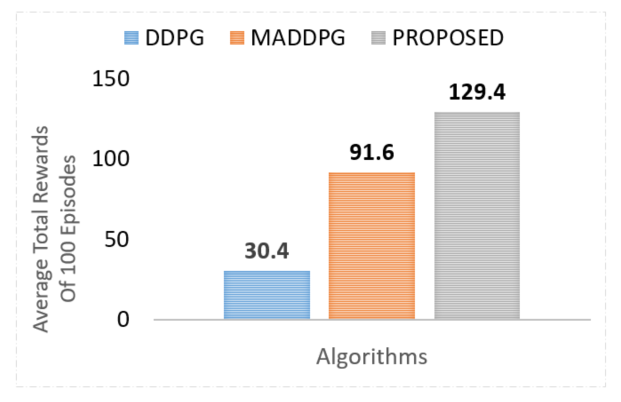
\includegraphics[width=8cm]{imgs/result_table.PNG}
  \caption{ Comparison result of 3 algorithms }
  \label{fig:result}
 \end{center}
\end{figure}

From Fig. \ref{fig:result}, our proposed method has an average reward of 129.4 over MADDPG's 91.6 and DDPG's 30.4, resulting in 41.3\% improvement over MADDPG and 325.7\% improvement over DDPG.

\section{Conclusion}
In this work, there are two problems in multi-agent task, one is that traditional RL methods can't solve multi-agent task because environment becomes non-stationary during learning and learning cannot converge, the second one is that random sampling batch data from experience replay is efficient for learning. We introduced our proposed method - Distributed Multi-Agent Cooperation Algorithm based on MADDPG algorithm using prioritized batch data in solving Predator-Prey task. Experiments shows we have 41.3\% improvement over MADDPG and 325.7\% improvement over DDPG. \par
Hyperparameters tuning and network architecture choice still remain a lot of work to do.
And due to current limited hardware resources, our experiments cost a lot time in training. This could be improved in future.

\section*{謝辞}
筑波大学大学院システム情報工学研究科准教授延原肇先生には,本研究を実施する機会を戴き,
その遂行に当たり様々な面でご指導を頂き,本論文の細部にわたるご助言を頂き心より御礼申し上げます.
また,的確なアドバイスを頂きました,中内靖先生,星野准一先生にこの場をお借りして感謝申し上げます.
最後に,本研究に対して様々なご助言とご協力をいただきました,計算知能・マルチメディア研究室の皆様に心より感謝申し上げます.

\begin{thebibliography}{9}

\bibitem{alphago}
David Silver, Aja Huang, et al. Mastering the Game of Go with Deep Neural Networks and Tree Search. Nature, 529(7587):484–489, 2016.

\bibitem{alphagozero} 
David Silver, Julian Schrittwieser, et al. Mastering the game of Go without human knowledge. Nature, 550:354–359, 2017.

\bibitem{starcraft} 
DeepMind and Blizzard open StarCraft II as an AI research environment. https://deepmind.com/blog/deepmind-and-blizzard-open-starcraft-ii-ai-research-environment.

\bibitem{game}
 P. Peng, Q. Yuan, et al. \textsl{Multiagent bidirectionally-coordinated nets for learning to play starcraft combat games}. CoRR, abs/1703.10069, 2017.

\bibitem{robot}
L. Matignon, L. Jeanpierre, A.-I. Mouaddib, et al. \textsl{Coordinated multi-robot exploration under
communication constraints using decentralized markov decision processes}. In AAAI, 2012.

\bibitem{google}
DeepMind AI reduces google data centre cooling bill by 40. https://deepmind.com/blog/deepmind-ai-reduces-google-data-centre-cooling-bill-40/.

\bibitem{finance}
Hull, J. C. Options, \textsl{Futures and Other Derivatives (9th edition)}. Prentice Hall, 2014.

\bibitem{maddpg} 
R Lowe, Y Wu, A Tamar, et al. \textsl{Multi-Agent Actor-Critic for Mixed Cooperative-Competitive Environments}. arXiv:1706.02275v2, 2017.

\bibitem{cover-heuristic}
A Isaza, J Lu, et al. \textsl{A Cover-Based Approach to Multi-Agent Moving Target Pursuit}. AIIDE, 2008.

\bibitem{qlearning} 
Christopher JCH Watkins and Peter Dayan. \textsl{Q-Learning}. Machine Learning, 8(3-4):279–292, 1992.

\bibitem{pg} 
R. S. Sutton, D. A. McAllester, S. P. Singh, and Y. Mansour. \textsl{Policy gradient methods for rein-
forcement learning with function approximation}. In Advances in neural information processing systems, pages 1057–1063, 2000.

\bibitem{ddpg} 
Timothy P Lillicrap, Jonathan J Hunt, et al. \textsl{Continuous Control with Deep Reinforcement Learning}. In ICLR, 2016.

\bibitem{ppo} 
John Schulman, Filip Wolski, et al. \textsl{Proximal Policy Optimization Algorithms}. arXiv:1707.06347, 2017.

\bibitem{cover} 
Xiao Tang, Nobuhara Hajime. \textsl{Real-time Grid-based Multi-Agent Pursuing A Moving Target method}. the 79th national convention of IPSJ, 2016. 

\bibitem{dpg} 
David Silver, Guy Lever, et al. \textsl{Deterministic Policy Gradient Algorithms}. In ICML, 2014.

\bibitem{dqn} 
Volodymyr Mnih, Koray Kavukcuoglu, et al. \textsl{Human-Level Control through Deep Reinforcement Learning}. Nature, 518(7540):529–533, 2015.

\bibitem{replay} 
Long-Ji Lin. \textsl{Self-Improving Reactive Agents Based on Reinforcement Learning, Planning and Teaching}. Machine Learning, 8(3–4):293–321, 1992.

\bibitem{a3c} 
Volodymyr Mnih, Adria Puigdomenech Badia, et al. \textsl{Asynchronous Methods for Deep Reinforcement Learning}. In ICLR, 2016.

\bibitem{a2c} 
Jane X Wang, Zeb Kurth-Nelson, et al. \textsl{Learning to Reinforcement Learn}. In CogSci, 2017.

\bibitem{param}
Peter Henderson, Riashat Islam, et al. \textsl{Deep Reinforcement Learning that Matters}. arXiv:1709.06560, 2017.

\bibitem{gym}
https://github.com/openai/gym

\bibitem{ou}
Uhlenbeck, George E and Ornstein, Leonard S. \textsl{On the theory of the brownian motion}. Physical
review, 36(5):823, 1930.

\bibitem{adam}
Diederik P. Kingma, Jimmy Ba. \textsl{Adam: A Method for Stochastic Optimization}. arXiv:1412.6980, 2014.

\end{thebibliography}

\vspace{2zh}
\begin{minipage}{73mm}
 \begin{wrapfigure}[6]{l}[-4pt]{30mm} 
 \begin{center}
  \includegraphics[width=30mm]{face.eps}
 \end{center}
 \end{wrapfigure}
 \noindent 筑 \ 波 \ 太 \  郎\\\\
 筑波大学大学院システム情報工学研究科知能機能システム専攻所属
\end{minipage}
\clearpage

\begin{comment}

\end{comment}

\appendix
\begin{algorithm*}[ht]
\caption{Distributed Multi-Agent DDPG algorithm (Master)}
\begin{algorithmic}
\State {Initialize replay memory $\mathbb{D}$}
\For {$episode = 1$ to max-episodes}
  \State {Initialize a random process $\cal{N}$ for action exploration}
  \State {Receive initial observation state $s$}
  \For {$t = 1$ to max-episode-length}
    \State {for each agent $i$, select action $a_i = \mu_i(o_i) + \cal{N}$ w.r.t. the current policy and exploration}
    \State {Execute actions and observe reward $r$ and new state $s'$}
    \State {Store (${s, a, r, s'}$) in replay memory $\mathbb{D}$}
    \For {agent $i = 1$ to n}
      \State {Sample a random batch data of transitions (${s, a, r, s'}$) with M-size from $\mathbb{D}$}
      \State {Divide M-size batch data into M-size/N-size parts, each part has N-size batch data}
      \State {Send each N-size batch data to each worker}
      \State {Receive loss calculation result from workers}
      \State {Set $\arg\max_{batch}(loss)$ as training batch}
      \State {Set $y = r_i + \gamma{Q_i}(o_i, (\bar{a}_1, \bar{a}_2, \ldots, \bar{a}_i ,\ldots, \bar{a}_n)|_{\bar{a}_j = \bar{\mu}_j(o_j)})$}
      \State {Update critic by minimizing the loss $L(\theta_i) = E_{s,a,r,s'}[y - Q(o_i, a_1, a_2, \ldots, a_n)]$}
      \State {Update actor using the sampled policy gradient:
      $$
         \frac{\partial J(\theta^\mu_i)}{\partial \theta^\mu_i} = 
 \mathbb{E}[\frac{\partial Q(o_i, a_1, a_2, \ldots, a_i ,\ldots, a_n|\theta^Q_i)}{\partial a_i} \frac{\partial \mu_i(o_i|\theta^\mu_i)}{\partial \theta^\mu_i}]
      $$
      }
    \EndFor
    \State {Update target network parameters for each agent i:
      $$\bar{\theta^i} \leftarrow \tau \theta^i + (1 - \tau)\bar{\theta^i}$$
    }
  \EndFor
\EndFor
\end{algorithmic}
\end{algorithm*}

\begin{algorithm*}[ht]
\caption{Distributed Multi-Agent DDPG algorithm (Worker)}
\begin{algorithmic}
\For {$episode = 1$ to max-episodes}
  \For {$t = 1$ to max-episode-length}
    \State {Receive network parameters from Master}
    \For {agent $i = 1$ to n}
      \State {Receive batch data (${s, a, r, s'}$) of N-size from Master}
      \State {Set $y = r_i + \gamma{Q_i}(o_i, (\bar{a}_1, \bar{a}_2, \ldots, \bar{a}_i ,\ldots, \bar{a}_n)|_{\bar{a}_j = \bar{\mu}_j(o_j)})$}
      \State {Calculate loss $L(\theta_i) = E_{s,a,r,s'}[y - Q(s, a_1, a_2, \ldots, a_n)]$}
      \State {Send loss result to Master}
    \EndFor
  \EndFor
\EndFor
\end{algorithmic}
\end{algorithm*}

\end{document}